\documentclass[40pt,a4paper,UTF8]{ctexart}
\usepackage{amsmath}
\usepackage{graphicx}

\usepackage{float}

%输入带圈数字  eg:\textcircled{1}
\usepackage{fontspec,xunicode-addon}

%代码显示的包
\usepackage{listings}
\usepackage{xcolor}

%打出空心字母
\usepackage{amsfonts,amssymb}

%整体加粗
\usepackage{bm}

%公式按照章节标号
\numberwithin{equation}{section}

%长等号
\usepackage{extpfeil}

%注释用
\usepackage{comment}
%----------------------------------------------
%配置代码显示格式-掌握minted之前的替代品
%----------------------------------------------
\definecolor{codegreen}{rgb}{0,0.6,0}
\definecolor{codegray}{rgb}{0.5,0.5,0.5}
\definecolor{codepurple}{rgb}{0.58,0,0.82}
\definecolor{backcolour}{rgb}{0.95,0.95,0.92}

\lstdefinestyle{mystyle}{
	backgroundcolor=\color{backcolour},   
	commentstyle=\color{codegreen},
	keywordstyle=\color{magenta},
	numberstyle=\tiny\color{codegray},
	stringstyle=\color{codepurple},
	basicstyle=\ttfamily\footnotesize,
	breakatwhitespace=false,         
	breaklines=true,                 
	captionpos=b,                    
	keepspaces=true,                 
	numbers=left,                    
	numbersep=5pt,                  
	showspaces=false,                
	showstringspaces=false,
	showtabs=false,                  
	tabsize=2
}

\lstset{style=mystyle}



%-----------------------------------------------------------------------------------

\title{第四章作业}
\author{Student name: Francisrk}
\date{Due date: February 20th, 2022}

\begin{document}

\maketitle   %控制序列,能将在导言区中定义的标题、作者、日期按照预定的格式展现出来。

\section{第1题}
\paragraph{}
已阅。
\paragraph{}


\section{第2题}
\paragraph{}

在undistort\_image.cpp中加入以下代码:
\begin{lstlisting}[language=C++, caption=在undistort\_image.cpp]
            double X=0, Y=0, X_distorted=0, Y_distorted=0, r=0;
            X = (u - cx)/fx;
            Y = (v - cy)/fy;
            r = sqrt(X * X + Y * Y);
            X_distorted = X * (1 + k1 * r * r + k2 * r * r * r * r) + 2 * p1 * X * Y + p2 * (r * r + 2 * X * X);
            Y_distorted = Y * (1 + k1 * r * r + k2 * r * r * r * r) + p1 * (r * r + 2 * Y * Y) + 2 * p2 * X * Y;
            u_distorted = fx * X_distorted + cx;
            v_distorted = fy * Y_distorted + cy;
\end{lstlisting}

\begin{lstlisting}[language=C++, caption=工程/CMakeLists.txt]
cmake_minimum_required(VERSION 3.21)
project(T_1)
set(CMAKE_CXX_STANDARD 11)
find_package(OpenCV 3 REQUIRED)
add_executable(undistort_image undistort_image.cpp )
target_link_libraries(undistort_image ${OpenCV_LIBS})
\end{lstlisting}

去畸变前后的对比图如图2.1所示。
\begin{figure}[H]
\centering
\includegraphics[width=4.8in]{ch4_2_1.png} {图2.1 去畸变前后对比图}
\end{figure}
\paragraph{}




\section{第3题}
\paragraph{}
\subsection{请说明鱼眼相机相比于普通针孔相机在 SLAM 方面的优势}
鱼眼相机最重要的一个优势就是相比于普通针孔相机拥有更宽阔的视野。因此可以确保在一段时间里,尽可能多的视觉特征进入相机视野,从而提高对周围环境的感知能力。

\subsection{请整理并描述 OpenCV 中使用的鱼眼畸变模型(等距投影)是如何定义的,它与上题的畸变模型有何不同}
本部分参考\cite{ref1},鱼眼镜头一般是由十几个不同的透镜组合而成的,如下图所示,在成像的过程中,入射光线经过不同程度的折射,投影到尺寸有限的成像平面上,使得鱼眼镜头与普通镜头相比起来拥有了更大的视野范围。
\begin{figure}[H]
\centering
\includegraphics[width=4.8in]{ch4_3_2.png} {图3.1 鱼眼镜头原理图}
\end{figure}

在研究鱼眼相机成像时,可以将上面的镜头组简化为一个球面,如图3.2(b)所示,$O_1-X_cY_cZ_c$是相机坐标系,$O_2-xy$是成像平面。现实世界有一点P,入射角为$\theta$,如果按照普通相机的针孔相机模型,入射光线$PO_1$经过镜头后不改变路线,$P,O_1,p'$三点共线,$p'$为$P$的像;但是对于鱼眼相机,入射光线$PO_1$经过镜头后会发生折射,因此$P$的想点为$p$点,极坐标为$(r,\varphi)$。
\begin{figure}[H]
\centering
\includegraphics[width=4.8in]{ch4_3_3.png} {图3.2 成像原理图\_1}
\end{figure}

为了将尽可能大的场景投影到有限的图像平面内,鱼眼相机会按照一定的投影函数来设计,如图3.2(a)所示。根据投影函数的不同,鱼眼相机的设计模型大致能被分为五种:透视投影(即针孔相机模型)、等积投影、等距投影、体视投影、正交投影。
\begin{figure}[H]
\centering
\includegraphics[width=4.8in]{ch4_3_4.png} {图3.3 鱼眼模型投影分类}
\end{figure}

接下来介绍鱼眼镜头的成像过程:
 实际的镜头因为各种原因并不会精确的符合投影模型,为了方便鱼眼相机的标定,一般取$r$关于$\theta$泰勒展开式的前5项来近似鱼眼镜头的实际投影函数:
\begin{align}
r(\theta)\approx k_0\theta + k_1 \theta^3 + k_2\theta^5 + k_3\theta^7 + k_4\theta^9
\end{align}

\begin{figure}[H]
\centering
\includegraphics[width=4.8in]{ch4_3_5.png} {图3.4 鱼眼模型成像过程}
\end{figure}

设相机系下有一点$P(x,y,z)$,点$P(x,y,z)$如果按照针孔相机模型投影,则不存在畸变,像点为$P_0(a,b)$,不妨设$f=1$(最终可以求得$\frac{r_d}{r}$与f无关),可得$P_0坐标为$
\begin{equation}
\left\{
\begin{array}{l}
a = \frac{x}{z}\\
b = \frac{y}{z}\\
r^2=a^2+b^2\\
\theta = arctan(r)
\end{array}
\right.
\end{equation}

由于畸变的存在,$P_0$点畸变成$p'$点,$r$被压缩到$r_d$,实际的像点位置为$p'(x',y')$,有$|Op'|=r_d,|OP_0|=r$,结合等距离投影函数
\begin{align}
r(\theta)=f(\theta)\approx k_0\theta + k_1 \theta^3 + k_2\theta^5 + k_3\theta^7 + k_4\theta^9
\end{align}
其中$r^2=a^2+b^2$表示相机空间任一点$P$归一化平面上的像点$p$距离光心的距离$|OP_0|$,根据对顶角$\angle{P_0O_CO}=\theta$,且有
\begin{equation}
\left\{
\begin{array}{l}
tan(\theta)=\frac{r}{f}=r\\
tan(\theta_d)=\frac{r_d}{f}=r_d\\
\end{array}
\right.
\end{equation}
考虑到相机的成像CCD平面尺寸一般都是几毫米,焦距在几百毫米左右,所以相机实际成像过程中$\theta_d$ 通常很小,$k_0$可以取1,所以有
\begin{align}
tan(\theta_d)\approx \theta_d=r_d
&= k_0\theta + k_1 \theta^3 + k_2\theta^5 + k_3\theta^7 + k_4\theta^9 \notag \\
&= \theta(1+k_1\theta^2+k_2 \theta^4+k_3\theta^6+k_4\theta^8)
\end{align}
如图3.4,畸变后的坐标为$p'[x',y']$,由相似关系:
\begin{align}
\frac{\theta_d}{r}=\frac{r_d}{r}=\frac{x'}{a}=\frac{y'}{b}=scale
\end{align}

所以有
\begin{equation}
\left\{
\begin{array}{l}
x'=scale*a\\ 
y'=sclae * b
\end{array}
\right.
\end{equation}

再根据相机内参转换成像素坐标$[u,v]$
\begin{equation}
\left\{
\begin{array}{l}
u = f_x * x' + c_x\\
v = f_y * y' + c_y
\end{array}
\right.
\end{equation}

有的地方还说有个$\alpha$偏度系数,我不知道这个是怎么得来的。

小结:由像素坐标计算未畸变的归一化坐标->找到畸变后的坐标->转换到像素平面。

更进一步:鱼眼相机的成像过程是已知入射角$\theta$求出射角$\theta_d$
,而鱼眼相机的畸变矫正则是已知畸变后的像点位置$(x',y')$,求实际的入射角$\theta$。由于相机参数已知,可以根据(x',y')以及相机焦距求得$\theta_d$的值,所以畸变矫正的本质问题是求解关于$\theta$的一元高次方程:
\begin{align}
\theta_d = \theta(1+k_1\theta^2+k_2\theta^4+k_3\theta^6+k_4\theta^8)
\end{align}
其中$k_1,k_2,k_3,k_4$是畸变系数,由相机标定结果提供。常用的求解一元高次方程的方法有二分法、不动点迭代、牛顿迭代法。如使用牛顿法迭代求解:

\begin{equation}
\begin{array}{c}
f(\theta) = \theta (1+k_1\theta^2+k_2\theta^4+k_3\theta^6+k_4\theta^8)-\theta_d \\ 
\theta_0 = \theta_d \\
\theta_{n+1} = \theta_n - \frac{f(\theta_n)}{f'(\theta_n)}
\end{array}
\end{equation}


\subsection{完成 fisheye.cpp 文件中的内容。针对给定的图像,实现它的畸变校正。要求:通过手写方式实现,不允许调用 OpenCV 的 API}
核心代码如下所示:
\begin{lstlisting}[language=C++, caption=工程/CMakeLists.txt]
            //变到相机坐标系
            double x = (u - cx) / fx, y = (v - cy) / fy;
            double r = sqrt(x * x + y * y);
            double theta = atan(r);
            double theta_d = theta * (1 + k1 * pow(theta, 2) + k2 * pow(theta, 4) + k3 * pow(theta, 6) + k4 * pow(theta, 8));
            double scale = theta_d / r;
            double x_distorted = scale * x;
            double y_distorted = scale * y;
            //去畸变完之后再变换到像素
            double u_distorted = fx * x_distorted + cx;
            double v_distorted = fy * y_distorted + cy;
\end{lstlisting}

\begin{figure}[H]
\centering
\includegraphics[width=4.8in]{ch4_3_1.jpg} {图3.5 鱼眼模型去畸变之后的结果}
\end{figure}


\subsection{为什么在这张图像中,我们令畸变参数k1, . . . , k4 = 0,依然可以产生去畸变的效果?}
由投影函数
\begin{equation}
\theta_d = \theta (1+k_1\theta^2+k_2\theta^4+k_3\theta^6+k_4\theta^8)
\end{equation}
取泰勒展开前五项来近似鱼眼模型,$k_1\cdots k_4$取0,相当于只近似了第一项,$\theta_d$的一次向系数$k_0$可以取1,所以说仍然可以完成去畸变的操作。

\subsection{在鱼眼模型中,去畸变是否带来了图像内容的损失?如何避免这种图像内容上的损失呢?}
鱼眼图一般为圆形,边缘的信息被压缩的很密,经过去除畸变后原图中间的部分会被保留的很好,而边缘位置一般都会被拉伸的很严重、视觉效果差,所以通常会进行切除,因此肯定会带来图像内容的损失。增大去畸变时图像的尺寸,或者使用单目相机和鱼眼相机图像进行融合,补全丢失的信息。

\section{第4题}
理论部分:
\subsection{推导双目相机模型下,视差与XYZ坐标的关系式。请给出由像素坐标加视差u,v,d推导XYZ与已知XYZ推导u,v,d两个关系。}
双目相机成像模型如图4.1所示
\begin{figure}[H]
\centering
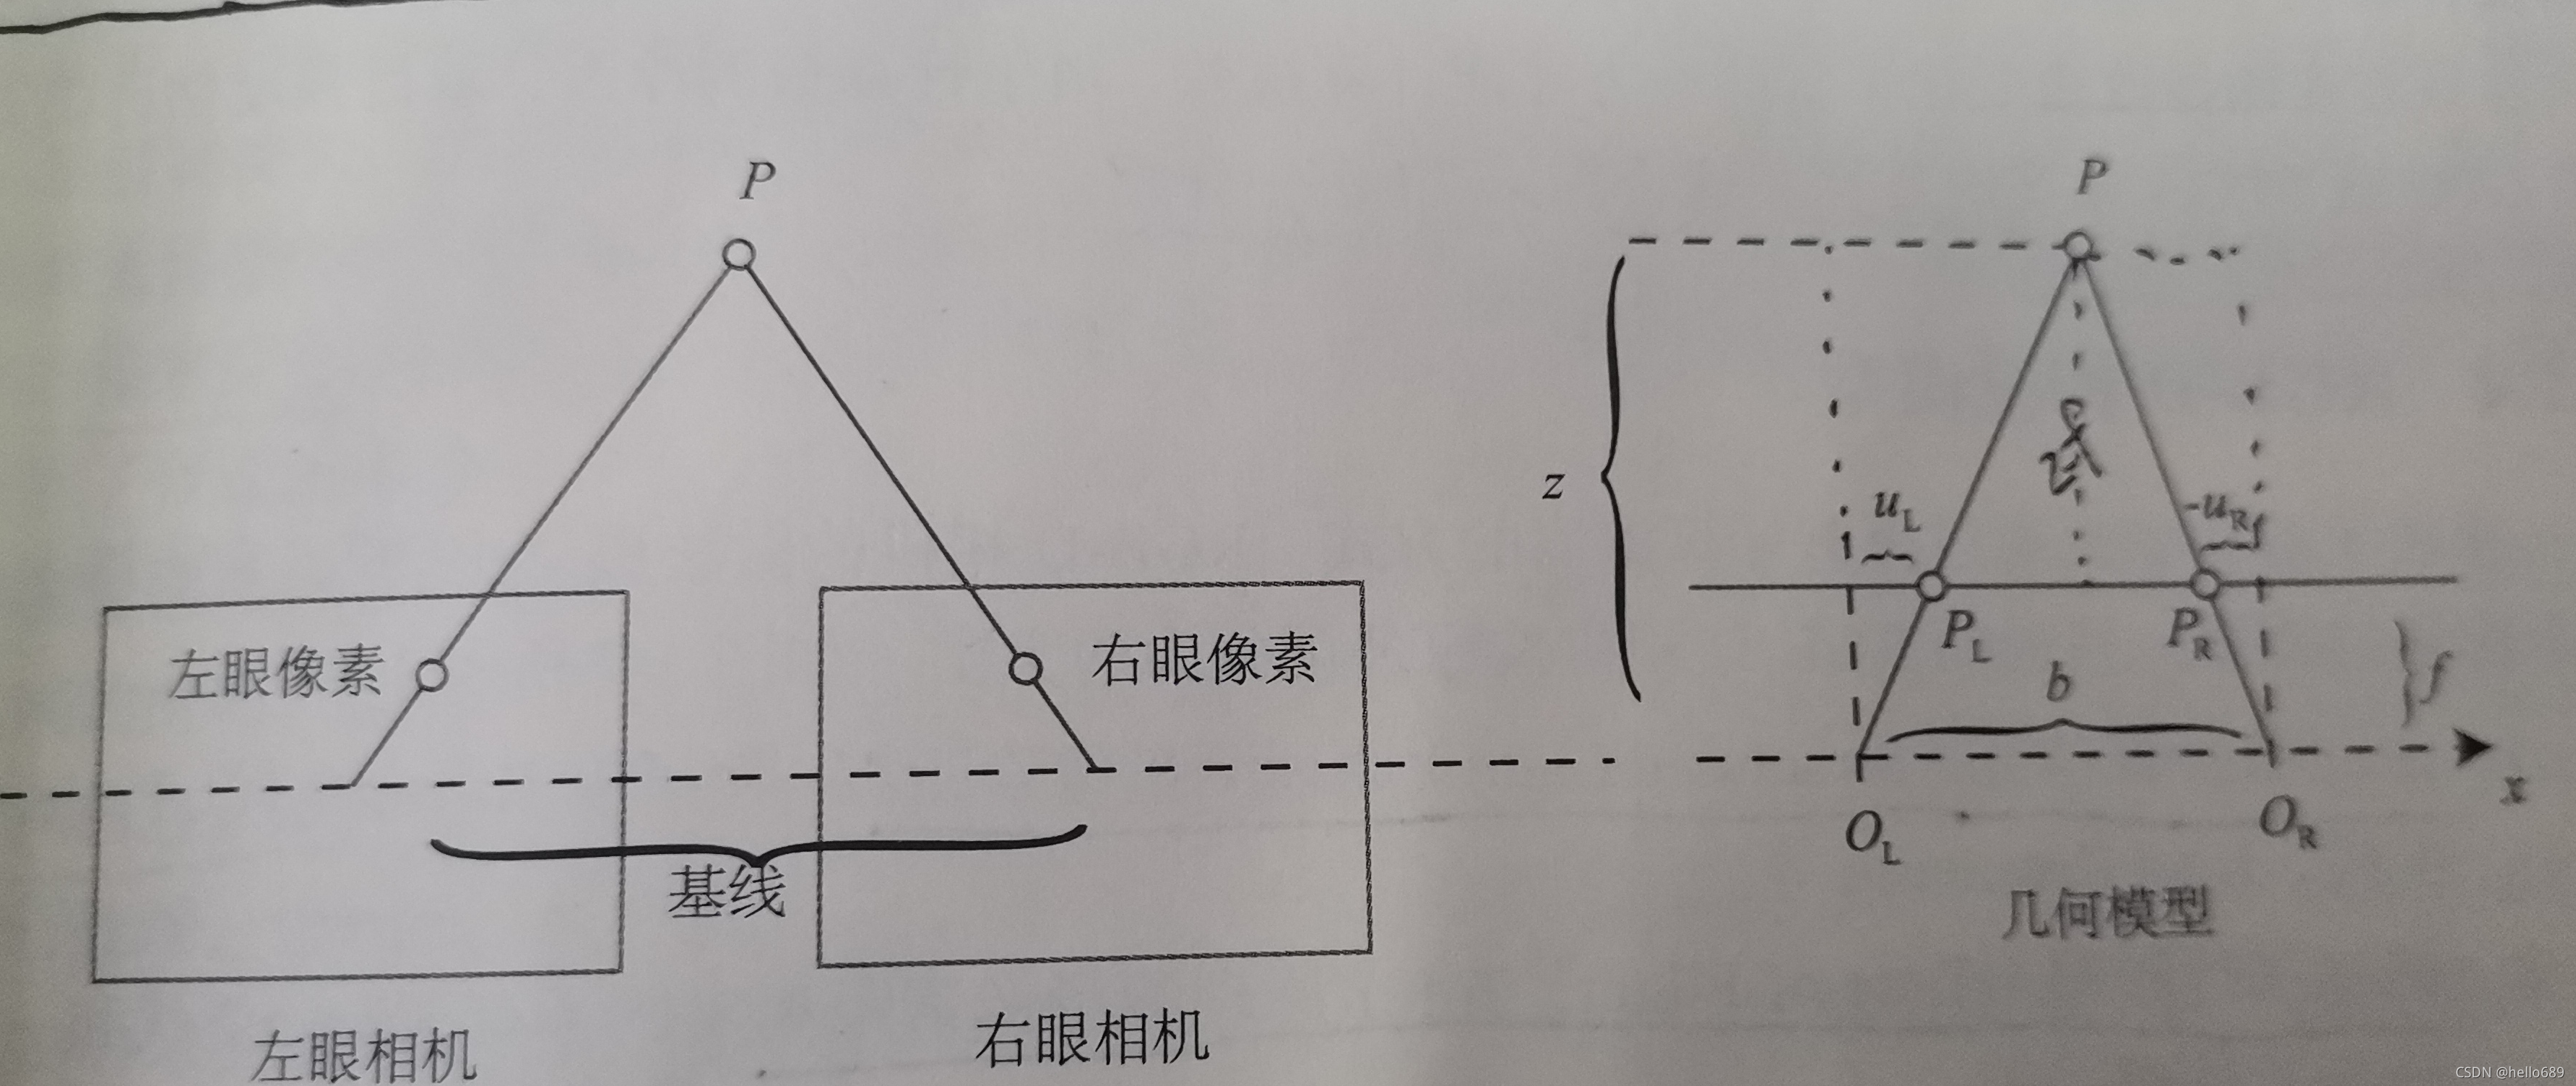
\includegraphics[width=4.8in]{ch4_4_1.png} {图4.1 双目相机成像模型}
\end{figure}

由$\Delta PP_LP_R$与$\Delta PO_LO_R$相似得

\begin{equation}
\frac{z-f}{z}=\frac{b-u_L+u_R}{b}
\end{equation}
其中焦距f,b基线是相机参数,已知。整理得:
\begin{equation}
z=\frac{fb}{d},d=u_L-u_R
\end{equation}
有针孔相机模型:
\begin{equation}
\left\{
\begin{array}{l}
u = f_x \frac{X}{Z}+c_x\\
v = f_y \frac{Y}{Z}+c_y
\end{array}
\right.
\end{equation}
所以当由u,v,d->X,Y,Z时,有:
\begin{equation}
\left\{
\begin{array}{l}
X=\frac{u-c_x}{f_x}*Z\\
Y=\frac{v-c_y}{f_y}*Z\\
Z=depth=\frac{fb}{d}
\end{array}
\right.
\end{equation}
当由X,Y,Z->u,v,d时,易得
\begin{equation}
\left\{
\begin{array}{l}
u = f_x \frac{X}{Z}+c_x\\
v = f_y \frac{Y}{Z}+c_y\\
d=\frac{fb}{Z}
\end{array}
\right.
\end{equation}
不过一般双目相机没有深度Z,所以需要借助双目深度恢复算法,如SGBM算法:
\begin{equation}
d=SGBM(X_{left},Y_{left},X_{Right},Y_{Right})
\end{equation}

\subsection{推导在右目相机下该模型将发生什么改变}
使用右眼相机坐标减去左眼相机坐标,$d=X_r-X_l$。使用右眼相机的投影点,另外使用左眼相机的外参。(这部分不太懂)




实践部分:
\subsection{根据双目图像和深度图绘制点云}
核心代码如下:
\begin{lstlisting}[language=C++, caption=工程/stereoVision.cpp]
            // start your code here (~6 lines)
            // 根据双目模型计算 point 的位置
            double x = (u - cx) / fx;  //和单目一样,只是这里可以计算深度信息,所以可以构建点云
            double y = (v - cy) / fy;
            double depth = fx * b / (disparity.at<uchar>(v, u));  //z=fb/d
            point[0] = x * depth;
            point[1] = y * depth;
            point[2] = depth;
            pointcloud.push_back(point);
            // end your code here
\end{lstlisting}

点云图如图4.2所示
\begin{figure}[H]
\centering
\includegraphics[width=4.8in]{ch4_4_2.png} {图4.2 双目生成点云图}
\end{figure}

\section{第5题}
\subsection{矩阵$\boldsymbol{A}\in \mathbb{R}^{N\times N}$,那么$d(\boldsymbol{Ax})/d\boldsymbol{x}$是什么?}
对于$\frac{\partial{(\bm{Ax})}}{\partial{\bm{x}}}$,记$\bm{f}=\bm{Ax}$,则对于向量微分:
\begin{equation}
d\bm{f}=(\frac{\partial{\bm{f}}}{\partial{\bm{x}}})^Td\bm{x}
\end{equation}
有:
\begin{align}
vec(d\bm{f})
&=d\bm f \notag \\
&=vec(\bm Ad \bm x) \notag \\
&=vec(\bm Ad\bm x \bm I_{1\times 1}) \notag \\
&=(\bm I_{1\times 1} \otimes \bm A)vec(d\bm x) \notag \\
&=\bm A d\bm x
\end{align}
对比(5.2)和(5.3)可得:
\begin{equation}
\frac{d(\boldsymbol{Ax})}{d\boldsymbol{x}}=
\frac{\partial{(\bm{Ax})}}{\partial{\bm{x}}}=\bm A^T
\end{equation}

\subsection{求$d(\bm{x^TAx})/d\bm x$}
由题目条件可知$f=\bm{x^TAx}$是标量函数,
\begin{align}
\frac{d(\boldsymbol{x^TAx})}{d\boldsymbol x}&= 
\frac{\partial{\boldsymbol{x^TAx}}}{\partial{\bm x}} \notag \\
&=
\frac{
(\partial \bm{x})^T\boldsymbol{Ax}+\boldsymbol{x}^T\boldsymbol{A}\partial \bm{x}
}
{d\boldsymbol{x}} \notag \\
&=\frac{\bm x^T \bm A^Td\bm x  + \bm x^T \bm A^T \bm d\bm x}{d\bm x} \notag \\
&=\bm x^T(\bm{A}+\bm{A}^T)
\end{align}

对于矩阵微分和迹有以下性质:
\begin{figure}[H]
\centering
\includegraphics[width=4.8in]{ch4_5_1.png}
\end{figure}
\begin{align}
(d\bm X)^T=d\bm X^T
\end{align}
当$\bm A$为常数矩阵时:
\begin{align}
d(\bm{XAX})^T=(d\bm{X})^T\bm{AX}^T+\bm{XA}(d\bm{X})^T
\end{align}
\begin{align}
d(\bm{X}^T\bm{AX})=(d\bm{X})^T\bm{AX}+\bm{X}^T\bm{A}d\bm{X}
\end{align}
对于$f=\bm{x^TAx}$有:
\begin{align}
df=tr(df)&=tr((d\bm{x})^T\bm{Ax}+\bm{x}^T\bm{A}d\bm{x}) \notag \\
&=tr((d\bm x)^T\bm{Ax})+tr(\bm{x}^T\bm{A}d\bm{x}) \notag \\
& \overset{tr(\bm AB)=tr(\bm BA)}{=}
tr((\bm{Ax})^Td\bm x)+tr(\bm{x}^T\bm{A}d\bm{x}) \notag \\
&=tr(((\bm{Ax})^T+\bm{x}^T\bm{A}) d\bm{x})
\end{align}
又由实值函数矩阵导数与微分的联系:
\begin{align}
df=tr(df)=tr((\frac{\partial f}{\partial \bm x})^Td\bm{x})
\end{align}
对比(5.8)和(5.9)得
\begin{align}
\frac{d(\boldsymbol{x^TAx})}{d\boldsymbol x}
&=\frac{\partial({\boldsymbol{x^TAx}})}{\partial{\bm x}}  \notag \\
&=\frac{\partial f}{\partial \bm x} \notag \\
&=((\bm{Ax})^T+\bm{x}^T\bm{A})^T \notag \\
&=\bm{Ax}+\bm{A}^T\bm{x} \notag \\
&=(\bm A+\bm A^T)\bm x
\end{align}


\subsection{证明$\bm{x^TAx}=tr(\bm{Axx^T})$}
证明如下:
\begin{align}
left&=\bm{x^TAx} \notag \\
&=
\begin{bmatrix}
x_1 & x_2 \cdots x_n 
\end{bmatrix}
\cdot
\begin{bmatrix}
a_{11} &a_{12}\cdots a_{1n} \\
a_{21} &a_{22}\cdots a_{2n} \\
\vdots &\ddots \\
a_{n1} & a_{n2}\cdots a_{nn}
\end{bmatrix}
\cdot
\begin{bmatrix}
x_1\\x_2\\\vdots \\x_n
\end{bmatrix}  \notag \\
&= x_1\sum\limits_{i=1}^{n}a_{1i}x_i + x_2\sum\limits_{i=1}^{n}a_{2i}x_i+\cdots +x_n\sum\limits_{i=1}^{n}a_{ni}x_i
\end{align}

\begin{align}
tr(\bm{Axx^T})
&=tr(
\begin{bmatrix}
a_{11} &a_{12}\cdots a_{1n} \\
a_{21} &a_{22}\cdots a_{2n} \\
\vdots &\ddots \\
a_{n1} & a_{n2}\cdots a_{nn}
\end{bmatrix} 
\cdot
\begin{bmatrix}
x_1\\x_2\\\vdots \\x_n
\end{bmatrix}
\cdot
\begin{bmatrix}
x_1&x_2&\cdots & x_n
\end{bmatrix}
 ) \notag \\
&=tr(
\begin{bmatrix}
a_{11} &a_{12}\cdots a_{1n} \\
a_{21} &a_{22}\cdots a_{2n} \\
\vdots &\ddots \\
a_{n1} & a_{n2}\cdots a_{nn}
\end{bmatrix}
\begin{bmatrix}
&x_1^2 & x_1x_2 & \cdots & x_1x_n  \\
&x_2x_1 & x_2^2 & \cdots & x_2x_n \\
& & & \vdots & \\
&x_nx_1 & x_nx_2 & \cdots & x_n^2
\end{bmatrix}
) \notag \\
&= x_1\sum\limits_{i=1}^{n}a_{1i}x_i + x_2\sum\limits_{i=1}^{n}a_{2i}x_i+\cdots +x_n\sum\limits_{i=1}^{n}a_{ni}x_i \notag \\
&=left
\end{align}
得证。


\section{第6题}
定义误差为:
\begin{equation}
e_i = y_i-exp(ax_i^2+bx_i+c)
\end{equation}
误差对每个状态变量求偏导,以构造雅可比:
\begin{equation}
\left\{
\begin{array}{l}
\frac{\partial{e_i}}{\partial a}=-x_i^2exp(ax_i^2+bx_i+c) \\
\frac{\partial{e_i}}{\partial b}=-x_iexp(ax_i^2+bx_i+c)  \\
\frac{\partial{e_i}}{\partial c}=-exp(ax_i^2+bx_i+c)
\end{array}
\right.
\end{equation}

核心代码如下所示:
\begin{lstlisting}[language=C++, caption=工程/gaussnewon.cpp]
        for (int i = 0; i < N; i++) {
            double xi = x_data[i], yi = y_data[i];  // 第i个数据点
            // start your code here
            double error = yi - exp(ae * xi * xi + be * xi + ce);  // 第i个数据点的计算误差
            Vector3d J; // 雅可比矩阵(是一个列向量)
            J[0] = -xi * xi * exp(ae * xi * xi + be * xi + ce);  // de/da
            J[1] = -xi * exp(ae * xi * xi + be * xi + ce);  // de/db
            J[2] = -exp(ae * xi * xi + be * xi + ce);  // de/dc
            //H△x=b
            H += J * J.transpose(); // GN近似的H
            b += -error * J;
            // end your code here

            cost += error * error;
        }

        // 求解线性方程 Hx=b,建议用ldlt
 	// start your code here
        Vector3d dx = H.ldlt().solve(b);  //MatrixBase的Cholesky分解求解线性方程组
	// end your code here
\end{lstlisting}

\begin{lstlisting}[language=bash, caption=工程/CMakeLists.txt]
cmake_minimum_required(VERSION 3.21)
project(T6)

set(CMAKE_CXX_STANDARD 11)

# OpenCV
find_package(OpenCV REQUIRED)
include_directories(${OpenCV_INCLUDE_DIRS})

# Eigen
include_directories("/usr/include/eigen3")

add_executable(gaussnewton gaussnewton.cpp)
target_link_libraries(gaussnewton ${OpenCV_LIBS})
\end{lstlisting}

\begin{figure}[H]
\centering
\includegraphics[width=4.8in]{ch4_6_1.png} {图6.1 手写高斯牛顿法结果}
\end{figure}

\section{第7题}
\subsection{给出H的具体形式}
此处的运动和观测方程和14讲P125中的方程不一样,此处有
\begin{equation}
\left\{
\begin{array}{l}
x_k = x_{k-1}+v_{k}+w_{k},  \quad\quad  \omega\thicksim \mathcal{N}(0,Q) \\
y_k = x_k+n_k, \quad \quad\quad\quad\quad n_k\thicksim \mathcal{N}(0,R) 
\end{array}
\right.
\end{equation}
其中
\begin{equation}
\left\{
\begin{array}{l}
e_{v,k}=v_k-(x_k-x_{k-1}) \\
e_{y,k}=y_k-x_k
\end{array}
\right.
\end{equation}
(14讲中的$e_{u,k}$定义反了,导致最后的$H$是错的。)
所以
\begin{align}
\bm{e_k}
&= 
\begin{bmatrix}
e_{v,k} \\
e_{y,k}
\end{bmatrix} \notag \\
&=\begin{bmatrix}
v_k-(x_k-x_{k-1})\\
y_k-x_k
\end{bmatrix} \notag \\
&=
\begin{bmatrix}
v_k\\y_k
\end{bmatrix}
-
\begin{bmatrix}
x_k-x_{k-1} \\
x_k
\end{bmatrix} \notag \\
&=\bm z_k-
\begin{bmatrix}
x_k-x_{k-1} \\
x_k
\end{bmatrix}
\end{align}

所以
\begin{align}
\bm e 
&=\begin{bmatrix}
\bm e_v\\ \bm e_y
\end{bmatrix} 
=\begin{bmatrix}
v_1\\v_2\\v_3\\y_1\\y_2\\y_3
\end{bmatrix}
-\begin{bmatrix}
x_1-x_0\\x_2-x_1\\x_3-x_2\\x_1\\x_2\\x_3
\end{bmatrix}
=\bm z-\bm H\bm x
\end{align}

由(7.4)得,$\bm H\in \mathbb{R}^{6\times 4}$所以
\begin{align}
\bm{Hx}=\bm{H}\cdot
\begin{bmatrix}
x_0\\x_1\\x_2\\x_3
\end{bmatrix}
=
\begin{bmatrix}
x_1-x_0\\x_2-x_1\\x_3-x_2\\x_1\\x_2\\x_3
\end{bmatrix}
\end{align}
结合$H$的维度可得
$$
\bm H = 
\begin{bmatrix}
-1&1&0&0\\
0&-1&1&0\\
0&0&-1&1\\
0&1&0&0\\
0&0&1&0\\
0&0&0&1
\end{bmatrix}
$$

\subsection{求$W$的具体取值}
由第1问可得:
转化为最小二乘问题:
\begin{align}
x^*
&=argmin\frac{1}{2}\bm{e}^TW^{-1}\bm{e} \notag \\
&=argmin(\frac{1}{2}(\sum\limits_{k=1}^{3}e_{v,k}^TQ_k^{-1}e_{v,k})+(\sum\limits_{k=1}^{3}e_{y,k}^TR_k^{-1}e_{y,k})) \notag \\
&=argmin(\frac{1}{2}
\begin{bmatrix}
e_{v,1}^T&e_{v,2}^T&e_{v,3}^T
\end{bmatrix}
\begin{bmatrix}
Q_1^{-1}& & \\
& Q_2^{-1}& \\
& & Q_3^{-1}
\end{bmatrix}
\begin{bmatrix}
e_{v,1}\\e_{v,2}\\e_{v,3}
\end{bmatrix}
+ \notag \\
& \quad 
\begin{bmatrix}
e_{y,1}^T&e_{y,2}^T&e_{y,3}^T
\end{bmatrix}
\begin{bmatrix}
R_1^{-1}& & \\
& R_2^{-1}& \\
& & R_3^{-1}
\end{bmatrix}
\begin{bmatrix}
e_{y,1}\\e_{y,2}\\e_{y,3}
\end{bmatrix} \notag \\
&=
argmin(\frac{1}{2})
\begin{bmatrix}
e_{v,1}\\e_{v,2}\\e_{v,3}\\e_{y,1}\\e_{y,2}\\e_{y,3}
\end{bmatrix}^T
\begin{bmatrix}
Q_1& &&&& \\
& Q_2&&&& \\
& & Q_3&&& \\
&&&R_1& & \\
&&&& R_2& \\
&&&& & R_3
\end{bmatrix}^{-1}
\begin{bmatrix}
e_{v,1}\\e_{v,2}\\e_{v,3}\\e_{y,1}\\e_{y,2}\\e_{y,3}
\end{bmatrix} \notag \\
&=argmin(\frac{1}{2}\bm{e}^T\bm W^{-1} \bm e
)
\end{align}
所以
\begin{align}
\bm W=diag(Q_1,Q_2,Q_3,R_1,R_2,R_3)
\end{align}

\subsection{是否有唯一解?}
是否有唯一解就看梯度下降时其系数矩阵的导数=0是否有唯一解,
\begin{figure}[H]
\centering
\includegraphics[width=4.8in]{ch4_7_1.png}
\end{figure}


\begin{thebibliography}{99}  
\bibitem{ref1}https://blog.csdn.net/qq\_16137569/article/details/112398976\#t5
\end{thebibliography}




\end{document}